\documentclass[]{article}
\usepackage{amsfonts, amssymb, amsmath}
\usepackage{float}
\usepackage{graphicx}

\title{Question 9.3.7}
\author{Anupama Kulshreshtha \\ EE22BTECH11009}
\date{}
\begin{document}
\maketitle
\providecommand{\pr}[1]{\ensuremath{\Pr\left(#1\right)}}
\providecommand{\prt}[2]{\ensuremath{p_{#1}^{\left(#2\right)} }}        % own macro for this question
\providecommand{\qfunc}[1]{\ensuremath{Q\left(#1\right)}}
\providecommand{\sbrak}[1]{\ensuremath{{}\left[#1\right]}}
\providecommand{\lsbrak}[1]{\ensuremath{{}\left[#1\right.}}
\providecommand{\rsbrak}[1]{\ensuremath{{}\left.#1\right]}}
\providecommand{\brak}[1]{\ensuremath{\left(#1\right)}}
\providecommand{\lbrak}[1]{\ensuremath{\left(#1\right.}}
\providecommand{\rbrak}[1]{\ensuremath{\left.#1\right)}}
\providecommand{\cbrak}[1]{\ensuremath{\left\{#1\right\}}}
\providecommand{\lcbrak}[1]{\ensuremath{\left\{#1\right.}}
\providecommand{\rcbrak}[1]{\ensuremath{\left.#1\right\}}}
\newcommand{\sgn}{\mathop{\mathrm{sgn}}}
\providecommand{\abs}[1]{\left\vert#1\right\vert}
\providecommand{\res}[1]{\Res\displaylimits_{#1}} 
\providecommand{\norm}[1]{\left\lVert#1\right\rVert}
%\providecommand{\norm}[1]{\lVert#1\rVert}
\providecommand{\mtx}[1]{\mathbf{#1}}
\providecommand{\mean}[1]{E\left[ #1 \right]}
\providecommand{\cond}[2]{#1\middle|#2}
\providecommand{\fourier}{\overset{\mathcal{F}}{ \rightleftharpoons}}
\newenvironment{amatrix}[1]{%
  \left(\begin{array}{@{}*{#1}{c}|c@{}}
}{%
  \end{array}\right)
}
%\providecommand{\hilbert}{\overset{\mathcal{H}}{ \rightleftharpoons}}
%\providecommand{\system}{\overset{\mathcal{H}}{ \longleftrightarrow}}
	%\newcommand{\solution}[2]{\textbf{Solution:}{#1}}
\newcommand{\solution}{\noindent \textbf{Solution: }}
\newcommand{\cosec}{\,\text{cosec}\,}
\providecommand{\dec}[2]{\ensuremath{\overset{#1}{\underset{#2}{\gtrless}}}}
\newcommand{\myvec}[1]{\ensuremath{\begin{pmatrix}#1\end{pmatrix}}}
\newcommand{\mydet}[1]{\ensuremath{\begin{vmatrix}#1\end{vmatrix}}}
\newcommand{\myaugvec}[2]{\ensuremath{\begin{amatrix}{#1}#2\end{amatrix}}}
\providecommand{\rank}{\text{rank}}
\providecommand{\pr}[1]{\ensuremath{\Pr\left(#1\right)}}
\providecommand{\qfunc}[1]{\ensuremath{Q\left(#1\right)}}
	\newcommand*{\permcomb}[4][0mu]{{{}^{#3}\mkern#1#2_{#4}}}
\newcommand*{\perm}[1][-3mu]{\permcomb[#1]{P}}
\newcommand*{\comb}[1][-1mu]{\permcomb[#1]{C}}
\providecommand{\qfunc}[1]{\ensuremath{Q\left(#1\right)}}
\providecommand{\gauss}[2]{\mathcal{N}\ensuremath{\left(#1,#2\right)}}
\providecommand{\diff}[2]{\ensuremath{\frac{d{#1}}{d{#2}}}}
\providecommand{\myceil}[1]{\left \lceil #1 \right \rceil }
\newcommand\figref{Fig.~\ref}
\newcommand\tabref{Table~\ref}
\newcommand{\sinc}{\,\text{sinc}\,}
\newcommand{\rect}{\,\text{rect}\,}
%%
%	%\newcommand{\solution}[2]{\textbf{Solution:}{#1}}
%\newcommand{\solution}{\noindent \textbf{Solution: }}
%\newcommand{\cosec}{\,\text{cosec}\,}
%\numberwithin{equation}{section}
%\numberwithin{equation}{subsection}
%\numberwithin{problem}{section}
%\numberwithin{definition}{section}
%\makeatletter
%\@addtoreset{figure}{problem}
%\makeatother

%\let\StandardTheFigure\thefigure
\let\vec\mathbf

There are 5\% defective items in a large bulk of items. What is the probability 
that a sample of 10 items will include not more than one defective item?
\solution
\begin{table}[!ht]
\centering
\begin{tabular}{|l|c|r|}
    \hline
    Parameter & Values & Description\\
    \hline
    $n$ & 10 & Number of items\\
    \hline
    $p$ & 0.05 & Probability of being defective\\
    \hline
    $q$ & 0.95 & Probability of not being defective\\
    \hline
    $X$ & 1 if defective & Bernoulli Random Variable\\
    {} & 0 if not defective & {}\\
    \hline
    $Y$ & $\sum_{i=1}^nX_i$ & Binomial Random Variable\\
    \hline
    $\mu = np$ & 0.5 & Mean\\
    \hline
    ${\sigma}^2 = npq$ & 0.475 & Variance\\
    \hline
\end{tabular}
\caption{Definition of parameters.}
\label{tab:gaussian/9/3/7}
\end{table}

The cdf using binomial is given by  
\begin{align}
	F_Y\brak{n} &= \Pr(Y \leq n) \\
        &= \sum_{k=0}^n\comb{10}{k}p^k\brak{1-p}^{10-k}
\end{align}
We require $\Pr(Y \leq 1)$. Since $n = 1$,
\begin{align}
	F_Y\brak{1} &= \Pr(Y \leq 1) \\
        &=  \sum_{k=0}^1\comb{10}{k}(0.05)^k\brak{0.95}^{10-k} \\
	&= 0.9138 
	\label{eq:9371}
\end{align} 
The gaussian distribution function is defined as:
\begin{align}
p_Y\brak{x} &= \frac{1}{\sqrt{2\pi{\sigma}^2}} e^{-\frac{\brak{x-\mu}^2}{2{\sigma}^2}}\label{9.3.8} \qquad \brak{x \in Y}
\end{align}
So,
\begin{align}
p_Y\brak{0} &= \frac{1}{\sqrt{2\pi\brak{0.475}}} e^{-\frac{\brak{0 - 0.5}^2}{2\brak{0.475}}}\\
		   &= \frac{1}{\sqrt{2\pi\brak{0.475}}} e^{-\frac{5}{19}}\\
	           &= 0.4450
\end{align}
\begin{align}
p_Y\brak{1} &= \frac{1}{\sqrt{2\pi\brak{0.475}}} e^{-\frac{\brak{1 - 0.5}^2}{2\brak{0.475}}}\\
		   &= \frac{1}{\sqrt{2\pi\brak{0.475}}} e^{-\frac{5}{19}}\\
	           &= 0.4450
\end{align}
Hence required probability,
\begin{align}
	p_Y &= p_Y\brak{0} + p_Y\brak{1}\\
	    &= 0.8901
	    \label{eq:9372}
\end{align}
From \eqref{eq:9371} and \eqref{eq:9372}
\begin{align}
F_Y\brak{1}\approx p_Y
\end{align}
\begin{figure}[!ht]
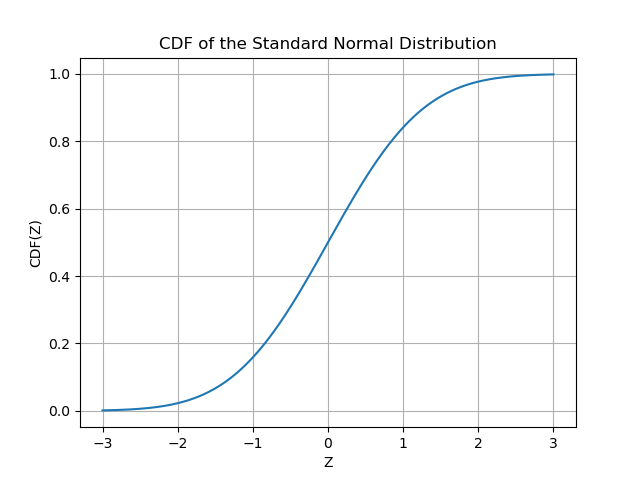
\includegraphics[width=\columnwidth]{./figs/fig.png}
\caption{Binomial pmf vs Gaussian pdf}
\label{fig:gaussian/9/3/7/}
\end{figure}
Solving using Q function\\
Q function is defined
\begin{align}
	\qfunc{x}=\int_x^{\infty}f\brak{x}dx
\end{align}
then CDF of $Y$ is:
\begin{align}
	\pr{Y<x}&=\int_{-\infty}^x f\brak{x} dx\\
	&=1-\int_x^{\infty}f\brak{x}dx\\
	&=1-\qfunc{x}
\end{align}
and for finding \pr{\frac{X-\mu}{\sigma}} Using approximation,
\begin{align}
	\pr{\frac{Y-\mu}{\sigma}} &\approx \pr{\frac{Y+0.5-\mu}{\sigma} < \frac{Y-\mu}{\sigma} < \frac{Y-0.5-\mu}{\sigma}}\\
	&\approx \pr{\frac{Y-\mu}{\sigma}<\frac{Y+0.5-\mu}{\sigma}} - \pr{\frac{Y-\mu}{\sigma}<\frac{Y-0.5-\mu}{\sigma}}\\
	&\approx \qfunc{\frac{Y-0.5-\mu}{\sigma}} - \qfunc{\frac{Y+0.5-\mu}{\sigma}}
\end{align}
\begin{align}
Y &= 1\\
\pr{Z=1.053} &\approx \qfunc{0} - \qfunc{1.45}\\
	       &\approx 0.4265
\end{align}
\end{document}
